\section{Auswertung}
\label{sec:Auswertung} 
\subsection{Untersuchung der Verzögerungszeiten}
\label{subsec:1}

Die Abhängigkeit der Anzahl der Impulse von der Verzögerungszeit wird durch Variation der Verzögerungszeit $T_{VZ}$ untersucht. Dabei wird die Anzahl der Impulse für die jeweilige Verzögerungszeit $T_{VZ}$ gemessen. Die aufgenommenen Messwerte sind in Tabelle \ref{tab:table1} zu sehen. In dem folgenden Diagramm \ref{fig:plot1} wird die Zahl der Impulse gegen die Verzögerungszeit $T_{VZ}$ aufgetragen. 

\begin{table}[H]
\centering
\caption{Anzahl gemessener Impulse für verschiedene Verzögerungszeiten $T_{VZ}$.}
\begin{tabular}{c|c||c|c}
$T_{VZ}/\mathrm{ns}$ & Impulse & $T_{VZ}/\mathrm{ns}$ & Impulse\\
\hline
-8	&   15 & 0 & 183\\
-7	&	63 & 1 & 169\\
-6	&	75 & 2 & 160\\
-5	&	95 & 3 & 148\\
-4	&	133& 4 & 134\\
-3	&	126& 5 & 134\\
-2	&	160& 6 &  87\\
-1	&	171& 7 &  82\\
 	&	   & 8 &  65\\
\label{tab:table1}
\end{tabular}
\end{table}

\begin{figure}[H]
 \centering
 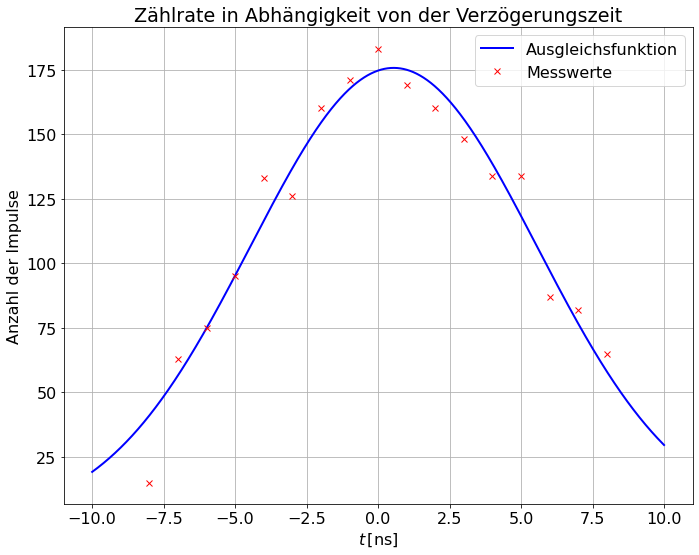
\includegraphics[width=0.75\textwidth]{plot1.png}
 \caption{Ausgleichsrechnung der verzögerungszeit-abhängigen Zählrate.}
 \label{fig:plot1}
\end{figure}

\newpage

\noindent Die zur Untersuchung der Verzögerungszeit $T_{VZ}$ verwendete Ausgleichsfunktion hat die Form

\begin{center}
$N = A \cdot e^{\frac{-(T_{VZ}-T_{VZ,0})^2}{2B^2}}$,
\end{center}

\noindent dessen Parameter mit Python 3 berechnet wurden. Die Parameter die sich durch die Ausgleichsrechnung zum fitten der Messwerte ergeben haben, lauten:

\begin{table}[H]
\centering
\begin{tabular}{lll}
$A$        &=& $176  \pm 5$    \\
$B$        &=& $(5,01 \pm 0,20)\,\mathrm{ns}$ \\
$T_{VZ,0}$ &=& $(0,54 \pm 0,17)\,\mathrm{ns}$ \\
\end{tabular}
\end{table}

\subsection{Bestimmung der Untergrundrate}
\label{subsec:2}

\noindent Die Gesamtzahl der Startsignale während eine Messdauer von $t_{ges}=272190\,\mathrm{s}$ beträgt $N_{start}=3256768$. Dabei beträgt die Dauer der Suchzeit $T_{s}=15\,\mathrm{ns}$ bei einer Kanalanzahl von $N_{Kanaele}=460$. \newline
\noindent Es soll die Untergrundrate (siehe Kapitel \ref{sec:Untergrundrate}) bestimmt werden. Dazu wird erst die Anzahl der Myonen berechnet, welche in der Suchzeit $T_{s}$ den Szintillator durchqueren, welche sich durch die folgende Formel berechnen lässt zu

\begin{center}
$\nu = \frac{N_{start}}{t_{ges}}=11,97\,\mathrm{\frac{1}{s}} .$
\end{center}

\noindent Nun wird die Wahrscheinlichkeit berechnet, dass ein weiteres Myon in den Szintillator tritt. Da diese poisson-verteilt sind ergibt sich die Wahrscheinlichkeit durch die folgende Formel zu

\begin{center}
$P = T_{s}\cdot \nu \cdot e^{T_{s} \cdot \nu} = 0,018\,\mathrm{\%} $
\end{center} 

\noindent Um die Anzahl der Fehlmessungen zu erhalten, wird die Wahrscheinlichkeit $P$ mit der Gesamtzahl der Startimpulse $N_{start}$ multipliziert. Damit ergibt sich für die Anzahl der Fehlmessungen bei einer Gesamtzahl an Startimpulsen $N_{start}$

\begin{center}
$N_{U}=N_{start}\cdot P= 584,62$
\end{center}

\noindent Um nun die Untergrundrate pro Kanal zu erhalten wird die Anzahl der Fehlmessungen noch durch die Anzahl der Kanäle dividiert. Damit ergibt sich eine Untergrundrate von 

\begin{center}
$U=\frac{N_U}{N_{Kanaele}}=1,27$ pro Kanal
\end{center}

\subsection{Zeit-Kanal Kalibrierung}
\label{subsec:3}

\noindent Um im nächsten Schritt die Lebensdauer des Myons bestimmen zu könne, ist eine Zeit-Kanal Kalibrierung notwendig. Dazu wird aufgenommen in welchem Kanal ein Impuls für verschiedene Doppelpulsabstände registriert wird. Diese Messwerte sind in Tabelle \ref{tab:table2} zu sehen.

\begin{table}[H]
\centering
\caption{Kanäle in denen ein Impuls für verschiedene Doppelpulsabstände registriert wurde.}
\begin{tabular}{c|c}
Kanal & $t/\mathrm{µs}$ \\
\hline
37		&0,8 \\
81		&1,8 \\ 
126		&2,8 \\
171		&3,8 \\
216		&4,8 \\
261		&5,8 \\
306		&6,8 \\
350		&7,8 \\
395		&8,8 \\
440		&9,8 \\
\label{tab:table2}
\end{tabular}
\end{table}

\begin{figure}[H]
 \centering
 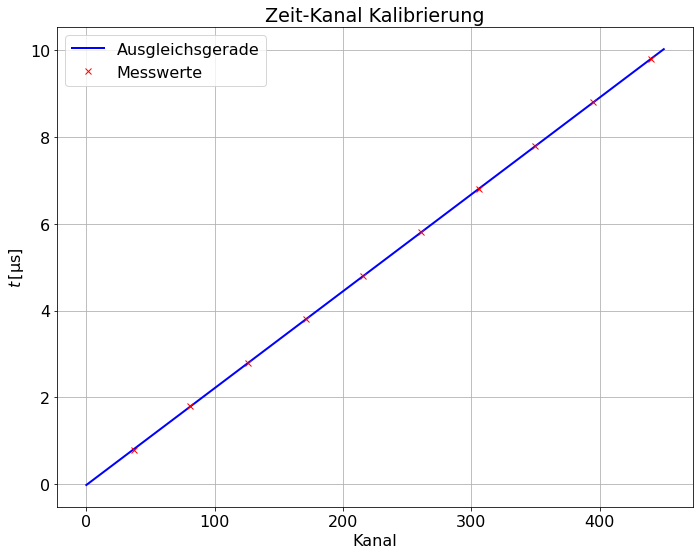
\includegraphics[width=0.75\textwidth]{plot2.png}
 \caption{Ausgleichsrechnung der Kanal-Zeit Kalibrierung.}
 \label{fig:plot2}
\end{figure}

\noindent Die Ausgleichsfunktion, die im Diagramm \eqref{fig:plot2} dargestellt ist, hat die Form

\begin{center}
$t = A \cdot K+B$,
\end{center}

\noindent dessen Parameter mit Python 3 berechnet wurden. Die Parameter die sich durch die Ausgleichsrechnung zum fitten der Messwerte ergeben haben, lauten:

\begin{table}[H]
\centering
\begin{tabular}{lll}
$A$   &=& $(0,022312 \pm 0,000018)\,$Kanal$\cdot\mathrm{µs}$    \\
$B$   &=& $(-0,017 \pm 0,005)\,\mathrm{µs} .$ \\
\end{tabular}
\end{table}

\subsection{Bestimmung der Lebensdauer}
\label{subsec:4}

\noindent Mithilfe der in Kapitel \ref{subsec:3} bestimmten Zeit-Kanal Kalibrierung kann nun die Lebensdauer $\tau$ bestimmt werden. Es wurde die Anzahl der gemessenen Start-Stopp Signale pro Kanal aufgenommen, um zusammen mit der Zeit-Kanal Kalibrierung eine Ausgleichsrechnung durchzuführen. 

\begin{figure}[H]
 \centering
 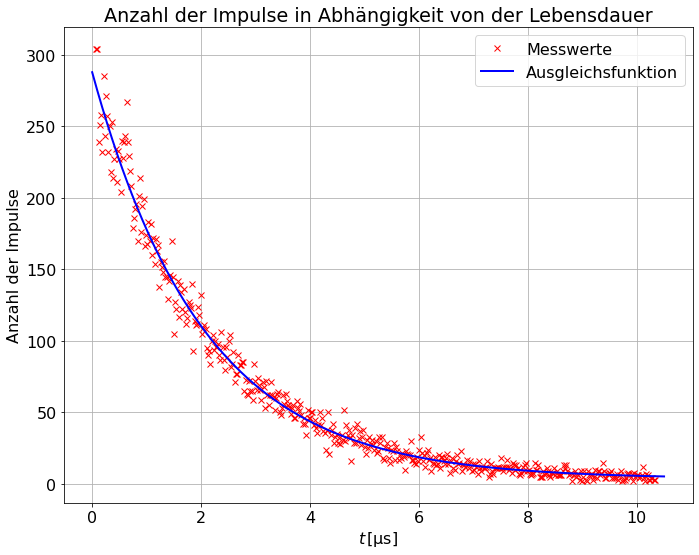
\includegraphics[width=0.75\textwidth]{plot3.png}
 \caption{Ausgleichsrechnung zur Bestimmung der Lebensdauer $\tau$.}
 \label{fig:plot3}
\end{figure}

\noindent Die Ausgleichsfunktion hat die Form

\begin{center}
$N = N_0\cdot e^{\frac{-t}{\tau}} + U\quad$, $\qquad$ mit $\quad t = A \cdot K+B$
\end{center}

\noindent dessen Parameter mit Python 3 berechnet wurden. Die Parameter die sich durch die Ausgleichsrechnung zum fitten der Messwerte ergeben haben, lauten:

\begin{table}[H]
\centering
\begin{tabular}{lll}
$N_0$   &=& $284,1\pm1,9  $ \\
$U$     &=& $  3,7\pm0,8  $ \\
\end{tabular}
\end{table}

\noindent Die Lebensdauer des Myons soll hierbei bestimmt werden. Wie bereits in Kapitel \ref{sec:Lebensdauer} erwähnt, ist $\symup{\tau}$ der entscheidende Parameter. Die experimentell bestimmte Lebensdauer $\tau$ des Myons lautet also:

\begin{table}[H]
\centering
\begin{tabular}{lll}
$\tau$  &=& $(2,043\pm0,028)\,\mathrm{µs}$ \\
\end{tabular}
\end{table}
